\section{Adam Bojek}
\label{sec:adambojek}

\subsection*{Suma i iloczyn}
Suma i iloczyn zbioru liczb od 1 do n:
\[
\sum_{i=1}^{n} i = \frac{n(n+1)}{2}
\]
\[
\prod_{i=1}^{n} i = n!
\]

\subsection*{Granica}
Przykład granicy:
\begin{equation}
\lim_{x \to \infty} \frac{1}{x} = 0
\end{equation}

\subsection*{Funkcja trygonometryczna}
Wzór na sinus podwojonego kąta:
\begin{equation}
\sin(2\theta) = 2 \sin(\theta) \cos(\theta)
\end{equation}
\textbf{Najlepsze sposoby na zabicie czasu na wykładzie}
\begin{itemize}
    \item \href{https://www.nytimes.com/games/wordle/index.html}{Wordle}
    \item \href{https://www.nytimes.com/games/connections}{Connections}
    \item \href{https://nerdlegame.com/}{Nerdle}
    \item \href{https://globle-game.com/}{Globle}
    \item Saper
    \item Spider Solitaire
    \item \href{https://www.netacad.com/}{Cisco Netacad}
\end{itemize}

\noindent \textbf{Ranking języków programowania}
\begin{enumerate}
    \item \textbf{Python}
    \item \textbf{JavaScript}
    \item \textbf{Java}
    \item \textbf{C++}
    \item \textbf{C\#}
\end{enumerate}

\noindent \textbf{Pingwin królewski} \textit{(Aptenodytes patagonicus)} – gatunek dużego nielotnego ptaka wodnego z rodziny pingwinów \textit{(Spheniscidae)}, zamieszkujący chłodne oceany półkuli południowej. Gnieździ się na obrzeżach \underline{Antarktydy}, Ziemi Ognistej, Falklandach i innych wyspach tej części świata. Jeden z najbardziej znanych gatunków pingwinów, zaraz po pingwinie cesarskim.
\subsection*{Cechy gatunku}
Wśród pingwinów drugi pod względem wielkości (po pingwinie cesarskim). Między płciami nie ma różnic w ubarwieniu. Upierzenie na szyi i barkach jasnoszare, na grzbiecie ciemnoszare z granatowym połyskiem. Policzki i gardło pomarańczowe, brzuch biały. Boki dzioba różowe, pozostałe części czarne. Pisklęta są brązowe, czasami bladopomarańczowe aż do pierzenia.
\subsection*{Wymiary średnie}
długość ciała ok. 90 cm (z ogonem)
masa ciała ok. 11–15 kg; samce nieco większe od samic
\subsection*{Wysiadywanie}
Jajo jest wysiadywane na zmianę przez samca i samicę przez ok. 55 dni. Rodzice trzymają jajo na stopach i przykrywają fałdą brzuszną. Zmieniają się co 6–18 dni; to z nich, które nie wysiaduje, płynie żerować. Po wykluciu pisklęta są jeszcze trzymane na stopach rodziców przez 30–40 dni, aż wykształcą puch i będą zdolne regulować temperaturę ciała.

\noindent Odwołanie do obrazka\ref{fig:pingwin}

\noindent Odwołanie do tabeli \ref{tab:porownanie_pingwinow}


\begin{table}[h!]
    \centering
    \begin{tabular}{|c|c|c|}
        \hline
        \textbf{Gatunek} & \textbf{Średni rozmiar} & \textbf{Miejsce występowania} \\
        \hline
        Pingwin cesarski & 115 cm & Antarktyda \\
        \hline
        Pingwin królewski & 90 cm & Subantarktyczne wyspy \\
        \hline
        Pingwin Adeli & 70 cm & Antarktyka \\
        \hline
        Pingwin białobrewy & 75 cm & Falklandy, subantarktyczne wyspy \\
        \hline
        Pingwin mały & 33 cm & Australia, Nowa Zelandia \\
        \hline
        Pingwin maskowy & 68 cm & Wyspa Georgia Południowa, Antarktyka \\
        \hline
    \end{tabular}
    \caption{Porównanie wybranych gatunków pingwinów według rozmiaru i miejsca występowania}
    \label{tab:porownanie_pingwinow}
\end{table}
\begin{figure}[htbp]
    \centering
    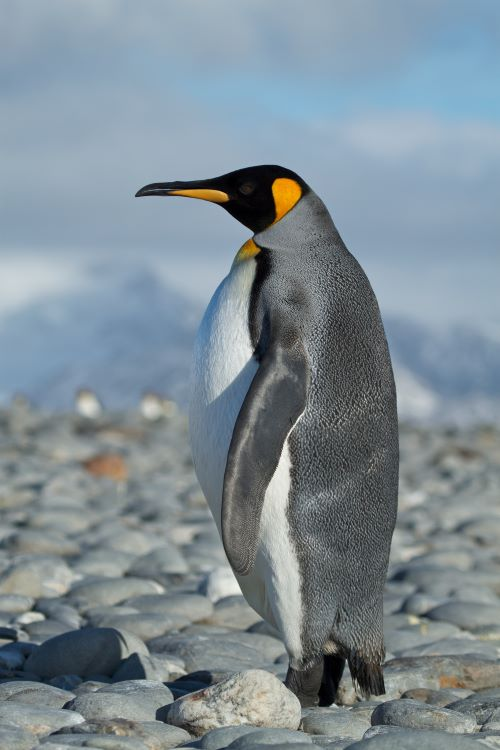
\includegraphics[width=0.25\textwidth]{pictures/pingwin.jpg}
    \caption{Pingwin}
    \label{fig:pingwin}
\end{figure}
